\documentclass[a4paper,10pt]{article}

\usepackage[utf8x]{inputenc}
\usepackage[ngerman]{babel}
\usepackage{graphicx}
\usepackage[a4paper,left=1.5cm,right=1.5cm,bottom=2cm,top=1cm]{geometry}
\usepackage{listings}
\lstset{inputencoding=utf8x, extendedchars=\true}

\usepackage{url}

\parindent 0pt
\parskip 10pt

\title{TTP1 - Protokoll}
\author{Andreas Krohn, Benjamin Vetter, Benjamin Jochheim}

\begin{document}

\maketitle

\tableofcontents 

\newpage

\section{Projektschritt 2: Vergleichende Betrachtung des B.A.T.M.A.N.- und OLSR-Protokolls}

\subsection{Welche Informationen tauschen die Nachbarn bei den jeweiligen Protokollen aus (Neighbor-Nachrichten)?}

% B.A.T.M.A.N.

\subsubsection*{B.A.T.M.A.N.}

B.A.T.M.A.N.-Nodes tauschen proaktiv sog. Originator-Nachrichten (OGMs) aus.
Eine OGM umfasst folgende Felder: 

\begin{description}
  \item[Version] Versionsnummer.
  \item[Is-direct-link flag] Kennzeichnet, ob der Knoten ein direkter Nachbar ist oder nicht.
  \item[Unidirectional flag] Kennzeichnet, ob der Knoten bidirektional ist oder nicht.
  \item[TTL] der Time-To-Live Wert der OGM.
  \item[GWFlags] Kennzeichnet ob der Originator als Gateway ins Internet fungiert. Ein Originator kann sich selbst als Internet-Gateway annoncieren. Die Annonce beinhaltet die Link-Geschwindigkeit.
  \item[GWPort] Beinhaltet eine Portnummer für einen Tunnel falls sich der Originator als Internet-Gateway annonciert.
  \item[Sequenznummer] Eine Sequenznummer der OGM (0 bis $2^{16}-1$). Anhand der Sequenznummer können andere Knoten entscheiden ob eine OGM "`neu"' ist.
  \item[Originator-Adresse] Die IP-Adresse des B.A.T.M.A.N. Interfaces des OGM-Initiators.
\end{description}

Einer OGM können sich Host Network Announcements (HNAs) anschließen. 
HNAs annoncieren ein Gateway zu einem Netzwerk oder Host.
Eine HNA umfasst folgende Felder: 

\begin{description}
  \item[Netmask] Kennzeichnet die Größe des annoncierten Netzes
  \item[Network address] Die Adresse des annoncierten Netzes
\end{description}

% OLSR

\subsubsection*{OLSR}

OLSR verfügt über ein generelles Messageformat.
Nachrichten können konkateniert werden.
Eine einzelne Nachricht besteht aus:

\begin{description}
  \item[Packet Length] Paketlänge.
  \item[Packet Sequence Number] Die Sequenznummer. Erhöht sich bei jeder neuen Nachricht um 1. 
  \item[Message Type] Die Message Type teilt mit um was für eine Nachricht es sich handelt, bzw. was das MESSAGE-Feld enthält.
  \item[Vtime] Die Validity Time teilt mit wie lange die Informationen das Pakets von einem Knoten als aktuell betrachtet werden sollen, sofern keine neuere Nachricht zu einem Update führt.
  \item[Message Size] Größe der Nachricht in Byte. Gezählt wird vom Feld Message Type an bis zum nächsten Message Type Feld (nächste konkaktenierte Nachricht).
  \item[Originator Address] Die Adresse des Knotens, der die Nachricht ursprünglich generiert hat.
  \item[Time To Live] Die maximale Anzahl an Hops. Der Wert wird dekrementiert bevor die Nachricht weitergeleitet wird.
  \item[Hop Count] Die Anzahl an Hops, die die Nachricht zurückgelegt hat.
  \item[Message Sequence Number] Der Originator einer Nachricht erzeugt eine eindeutige ID für jede Nachricht.
  \item[MESSAGE] Nachricht vom Typ \textbf{Message Type}
\end{description}

Anhand des Message Type Feldes wird festgelegt, welcher Nachrichtentyp im MESSAGE-Block enthalten ist. 
RFC3626 spezifiziert die Nachrichtentypen HELLO, TC, MID und HNA.

\begin{description}
  \item[HELLO] HELLO-Nachrichten erfüllen den Zweck der Veröffentlichung der lokalen Routinginformationen, dem Erkennen von Nachbarn und der Auswahl der Multipoint Relays. Daher werden HELLO-Nachrichten stets periodisch verschickt. Eine HELLO-Nachricht besteht aus einer Liste von bekannten Nachbaradressen und Informationen (Status des Nachbarn) über diese Nachbarn, sowie der eigenen Bereitschaft Pakete weiterzuleiten (Willingness).
  \item[TC] TC-Nachrichten dienen dazu die gewonnen Informationen über die Topologie zu verteilen. TC-Nachrichten werden von MPRs erstellt und beinhalten mindestens die Knoten von denen sie als MPR ausgewählt wurden.
  \item[MID] Knoten, die über mehrere OLSR Interfaces verfügen verschicken MID-Nachrichten um den anderen Knoten ihre Interfacekonfiguration mitzuteilen.
  \item[HNA] Knoten, die über Routinginformationen bzgl. der Außenwelt des MANETs betreffen, verschicken analog zu B.A.T.M.A.N. Host Network Announcement Nachrichten (HNAs).
\end{description}

\subsection{Wie ermitteln/bewerten sie die Qualität der Links}

% B.A.T.M.A.N.

\subsubsection*{B.A.T.M.A.N.}

Erhält ein Knoten schneller und zuverlässiger OGMs von einem Nachbarn kann er diesen Knoten als Best-Next-Hop auswählen um Nachrichten an weiter entfernte Knoten zu verschicken.
Hierzu unterhält jeder Knoten ein Sliding-Window bzgl. der Sequenznummern von OGMs jedes Nachbarn. 
Erhält ein Knoten eine OGM von einem Nachbarn betrachtet er die Sequenznummer der OGM.
Wenn die Sequenznummer im Fenster vorhanden ist, speichert der Knoten diese Information.
Hingegen wird das Fenster verschoben, wenn die Sequenznummer außerhalb des Fensters liegt.
Je mehr Sequenznummern innerhalb des Fensters liegen, desto besser bewertet der Knoten die Link-Qualität.
Der Link, der die meisten Sequenznummern in seinem Fenster aufweisen kann, gilt als aktueller Best-Next-Hop.

% OLSR

\subsubsection*{OLSR}

von AK zu bearbeiten

...RFC lesen..
Link Set über HELLO Messages aufbauen. Eigener Originator in 
empfangener Message enthalten -> Symmetrischer Link. Timeouts -> Asymmetrisch, dann Tot.
Symmetrie eines Links ist ein Indiz für Qualität.. bla..
Signal Noise Ratio -> l\_link\_quality P.57f

Der verwendete OLSR-Daemon nutzte Link Quality Extensions (ETX-metrik).
Das RFC-gemäße OLSR versucht nur die HOP-Distanz zu minimieren. Die Link-Qualität
wird nach RFC nicht berücksichtigt. Das kann bedeuten das ein unzuverlässiger Link zu einem Ziel bevorzugt wird,
wenn er eine geringere HOP-Distanz bietet.

Der um Link Quality Extensions erweiterte OLSR-Daemon wertet die erwarteten und tatsächlich empfangenen
HELLO Pakete seiner direkten Nachbarn aus und kann dadurch die Link-Qualität bestimmen.

http://www.olsr.org/docs/README-Link-Quality.html

\subsection{Wie bilden sich die lokalen Mesh-Konfigurationen?}

% B.A.T.M.A.N.

\subsubsection*{B.A.T.M.A.N.}

B.A.T.M.A.N. ist ein proaktives Routing-Protokoll.
Das Protokoll hat das Ziel für jeden Knoten den jeweils besten Next-Hop zu finden, so dass keine vollständigen Routen verwaltet werden müssen, sondern nur der nächste Hop zum Ziel.
Jeder Knoten broadcastet Originator-Nachrichten (OGMs) periodisch um seine Nachbarn über seine Existenz zu informieren.
Ein Jitter verhindert dabei Kollisionen.
Seine Nachbarn re-broadcasten die OGMs und informieren ihrerseits ihre Nachbarn über die Existenz des eigentlichen Absenders der OGM.
Jeder Knoten re-broadcastet die OGM seines aktuell als Best-Next-Hop identifizierten Knotens, sofern der Knoten die OGM anhand der Sequenznummer als "`neu"' einstuft und die TTL noch nicht abgelaufen ist.
Bei jedem Re-broadcasting wird der TTL-Wert um 1 verringert.
Daher wird das Netz mit OGMs geflutet.
Eine Verbindung mit einem spezifischen Nachbarn gilt als bidrektional wenn ein Knoten seine eigenen OGMs von diesem Nachbarn empfängt.

% OLSR

\subsubsection*{OLSR}
%von BJ zu bearbeiten
Das OLSR (Optimized Link State Routing) Protokoll ist ebenso wie B.A.T.M.A.N. ein proaktives Routingprotokoll.
OLSR wird in dem RFC3626 (aus dem Jahr 2003) beschrieben.

Bei OLSR ist allen Routern die Netztopologie vollständig bekannt. Ein Router benötigt daher im Vergleich zu B.A.T.M.A.N. bei größeren
Netzen wesentlich mehr Speicherplatz.
% Ist OLSR immer Loop-Frei ?
Die im Praktikum eingesetzte OLSR Software (von olsr.org) ist nicht RFC-Konform sondern wurde um einige dinge erweitert:

\begin{description}
\item[Linkqualität], die Linkqualität wird zur berechnung der Route herangezogen.
\item[ETX], Expected Transmission Count (eine Maßnahme zur feststellung der Linkqualität asymetrischer Links)
\item[Fish Eye Algorithmus], Routen zu weiter entfernten Knoten werden seltener neu berechnet, dadurch bessere Skalierbarkeit
\end{description}

\subsection{Ist das B.A.T.M.A.N.-Protokoll wirklich immer Loop-frei? Wie könnten sich ggf. Loops bilden?}

von BJ zu bearbeiten

Sind mehrere Nodes sowohl per BATMAN als auch per klassischem Ethernet verbunden, kann eine Loop entstehen.
Die BATMAN-spezifischen Paketheader werden im Ethernet nicht weitergeleitet, damit die Mechanismen zur Loopverhinderung ausgehebelt....
 Allerdings ist folgendes Szenario denkbar:
Bei schwankender Linkqualität könnte ein Paket mehrfach an einem Host ankommen.
In dem Bild

%loop-routing.eps einfuegen


möchte Host Z ein Paket an E senden. Dazu wählt er seinen nächsten Hop A aus.
Die beiden Verbindungen zum zielhost sind jedoch von schlechter qualität.
In dem moment in dem das Paket ankommt ist die Verbindung AE zusammengebrochen.
Daher sendet A das Paket an D.
D sendet an C.
In dem moment in dem C das Paket erhält bricht die Verbindung zu E zusammen, so daß C das Paket wieder an A sendet.
%etc.

Bei unseren Versuchen konnten wir solche Loops nicht erzeugen.

\section{Projektschritt 3: Vergleichende Analyse der Übertragungsqualität}

Unsere Access Points (APs) hatten die Nummbern 12 und 14, im weiteren als AP-12 und AP-14 bezeichnet.
Um vergleichbare, reproduzierbare und praxisrelevante Ergebnisse zu erhalten haben wir die Messungen zum größten Teil von Ende zu Ende durchgeführt, denn in der Praxis ist auch eher die Verbindungsqualität an den Endpunkten von Interesse.
Dazu haben wir bspw. die Ping- und Iperf-Messungen auf unseren Notebooks durchgeführt, die jeweils mit einem AP verbunden wurden.
Das 1. Notebook (Notebook-1) wurde mit dem AP-12 verbunden, das 2. Notebook (Notebook-2) wurde mit dem AP-14 verbunden.
Da die Untersuchungen für eine sensitive Echtzeitapplikation durchgeführt werden sollten, haben wir Messungen mit Iperf primär für UDP-Datenströme durchgeführt.

Um den Einfluss der Hop-Anzahl bemessen zu können haben wir die Messungen außerdem für zwei verschiende Szenarien durchgeführt:
\begin{itemize}
  \item[1-Hop] die kommunizierenden Endpunkte sind über ihre unterschiedlichen Access Points direkt miteinander verbunden 
  \item[Multi-Hop] die kommunizierenden Endpunkte sind über ihre unterschiedlichen Access Points und weitere, zusätzliche Hops (APs) miteinander verbunden
\end{itemize}

Wir haben uns dafür entschieden das zweite Szenario als "`Multi-Hop"' zu bezeichnen, da das B.A.T.M.A.N.-Protokoll nicht die genaue Netztopologie kennt, sondern nur den jeweils besten Next-Hop.
Dadurch ist nicht möglich die Anzahl an Hops genau zu bemessen oder festzulegen.

Um die Szenarien anschaulicher zu beschreiben lassen sich die Statistiken der Routing-Daemons abfragen.
Für B.A.T.M.A.N. wurde hierzu folgender Befehl benutzt:

\begin{lstlisting}
$ batmand -c -d 1
\end{lstlisting}

Für B.A.T.M.A.N. sieht unser 1-Hop-Szenario bspw. wie folgt aus (AP-12):

\begin{lstlisting}
Originator (#/255)    Nexthop [outgoingIF]:  Potential nexthops
10.0.0.14    (251)  10.0.0.14 [      eth2]:      10.0.0.14 (251) 
10.0.0.24    ( 25)  10.0.0.14 [      eth2]:      10.0.0.24 (  0)
10.0.0.53    ( 34)  10.0.0.53 [      eth2]:      10.0.0.53 ( 34) 
10.0.0.13    (  8)  10.0.0.53 [      eth2]:      10.0.0.53 (  8)  
\end{lstlisting}

Unser Best-Next-Hop um zu AP-14 zu gelangen ist AP-14 selbst, d.h. bei einer Kommunikation von AP-12 zu AP-14 liegt kein weiterer HOP dazwischen.

Für B.A.T.M.A.N. sieht unser Multi-Hop-Szenario bspw. wie folgt aus (AP-12):

\begin{lstlisting}
Originator (#/255)    Nexthop [outgoingIF]:   Potential nexthops
10.0.0.14    ( 32)  10.0.0.53 [      eth2]:       10.0.0.53 ( 32)
10.0.0.24    ( 29)  10.0.0.53 [      eth2]:       10.0.0.53 ( 29)
10.0.0.53    ( 44)  10.0.0.53 [      eth2]:       10.0.0.53 ( 44)
10.0.0.13    ( 42)  10.0.0.53 [      eth2]:       10.0.0.53 ( 42)
\end{lstlisting}

Unser Best-Next-Hop um zu AP-14 zu gelangen ist AP-53, d.h. bei einer Kommunikation von AP-12 zu AP-14 liegt mindstens 1 weiterer Hop dazwischen.

Um den OLSR-Routing-Daemon nach seinen Routing-Entscheidungen zu befragen haben wir das OLSR-HttpInfo-Modul benutzt.

Abbildung \ref{1hop_olsr} zeigt die Routing-Informationen für OLSR bzgl. des 1-Hop-Szenarios (AP-12).

\begin{center}
  \begin{figure}[thb]
    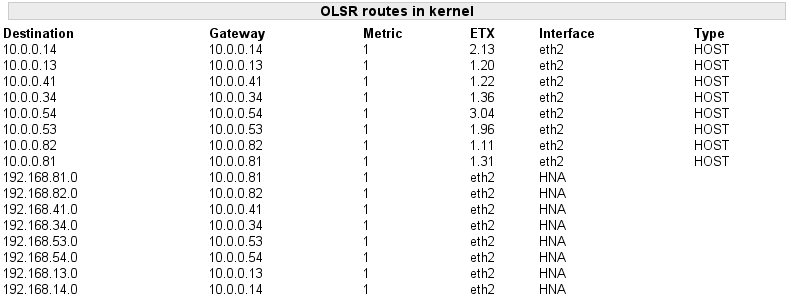
\includegraphics[width=1\textwidth]{1hop_olsr.png}
    \caption{1-Hop OLSR}
    \label{1hop_olsr}
  \end{figure}
\end{center}

Unsere Route zu AP-14 weist die Metrik 1 auf und der Gateway zu AP-14 ist AP-14 selbst, d.h. bei einer Kommunikation von AP-12 zu AP-14 liegt kein weiterer Hop dazwischen.

Figure \ref{2hop_olsr} zeigt die Routing-Informationen für OLSR bzgl. des Multi-Hop-Szenarios (AP-12).

\begin{center}
  \begin{figure}[thb]
    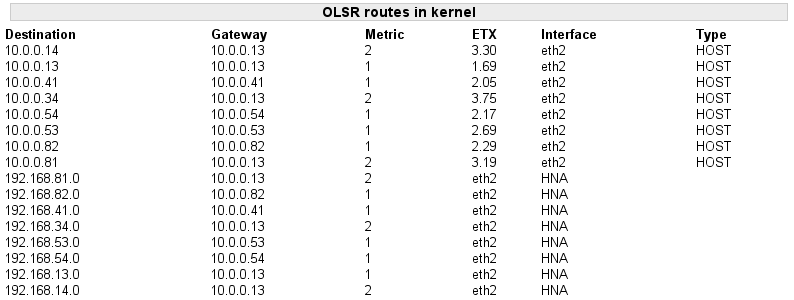
\includegraphics[width=1\textwidth]{2hop_olsr.png}
    \caption{Multi-Hop OLSR}
    \label{2hop_olsr}
  \end{figure}
\end{center}

Unsere Route zu AP-14 weist die Metrik 2 auf und der Gateway zu AP-14 ist AP-13, d.h. bei einer Kommunikation von AP-12 zu AP-14 liegt ein weiterer Hop (AP-13) dazwischen.

\subsubsection*{Hinweis bzgl. der Szenarien}

Da die APs ständig ihre Routing-Entscheidungen ändern können,
haben wir vor und während der Messungen immer überprüft ob das gerade zu untersuchende Szenario überhaupt (noch) vorhanden ist.

%http://openmaniak.com/iperf.php
%
%als erstes mal bandwidth check
%==============================
%
%\begin{lstlisting}
%server: iperf -s -u # udp server öffnen (ggf -i für periodische ausgabe)
%client: iperf -c [IP] -u -i -t [SECONDS] # client zum server per udp connecten und bandwidth check mit periodischer ausgabe
%\end{lstlisting}
%
%
%dann bidirectional bandwidth check:
%===================================
%
%\begin{lstlisting}
%client: iperf -c [IP] -u -r -i # client zum server per udp connected und bidirectional bandwidth check
%\end{lstlisting}
%
%dann simultaneous bidirectional bandwidth check
%===============================================
%
%\begin{lstlisting}
%client: iperf -c [IP] -u -d
%\end{lstlisting}
%
\subsection{1. Paketverluste (Loss)}

Die Paketverluste haben wir mittels Ping als auch mit Iperf gemessen.

\subsubsection{Paketverluste bzgl. B.A.T.M.A.N.}

\subsubsection*{1-Hop-Szenario}

Zunächst haben wir die Paketverluste bzgl. B.A.T.M.A.N. grob mittels Ping gemessen.

\begin{lstlisting}
root@AP-12:~# ping -c 20 10.0.0.14
PING 10.0.0.14 (10.0.0.14): 56 data bytes
64 bytes from 10.0.0.14: icmp_seq=1 ttl=64 time=3.9 ms
...

--- 10.0.0.14 ping statistics ---
20 packets transmitted, 19 packets received, 5% packet loss
round-trip min/avg/max = 3.0/9.9/59.7 ms
\end{lstlisting}

Die Messung mittels Ping ergab einen Paketverlust von 5\%.
Anschließend haben wir die Paketverluste bzgl. B.A.T.M.A.N. mittels Iperf gemessen.

\begin{lstlisting}
user@notebook-1:~$ iperf -s -u
------------------------------------------------------------
Server listening on UDP port 5001
Receiving 1470 byte datagrams
UDP buffer size:   122 KByte (default)
------------------------------------------------------------
[  3] local 192.168.12.139 port 5001 connected with 192.168.14.232 port 45829
[ ID] Interval       Transfer     Bandwidth       Jitter   Lost/Total Datagrams
[  3]  0.0-10.0 sec  1.25 MBytes  1.05 Mbits/sec  1.342 ms    3/  893 (0.34%)
[  4] local 192.168.12.139 port 5001 connected with 192.168.14.232 port 54231
[  4]  0.0-10.0 sec  1.25 MBytes  1.05 Mbits/sec  0.816 ms    2/  893 (0.22%)
[  3] local 192.168.12.139 port 5001 connected with 192.168.14.232 port 41070
[  3]  0.0-10.0 sec  1.25 MBytes  1.04 Mbits/sec  1.014 ms    4/  893 (0.45%)
[  4] local 192.168.12.139 port 5001 connected with 192.168.14.232 port 45941
[  4]  0.0-10.0 sec  1.25 MBytes  1.05 Mbits/sec  3.377 ms    2/  893 (0.22%)
[  3] local 192.168.12.139 port 5001 connected with 192.168.14.232 port 40947
[  3]  0.0-10.0 sec  1.25 MBytes  1.05 Mbits/sec  2.689 ms    0/  893 (0%)
[  4] local 192.168.12.139 port 5001 connected with 192.168.14.232 port 47410
[  4]  0.0-10.0 sec  1.25 MBytes  1.05 Mbits/sec  2.218 ms    0/  893 (0%)
\end{lstlisting}

Die Messungen mittels Iperf ergaben Paketverluste von $< 1\%$.

\subsubsection*{Multi-Hop-Szenario}

Auch für das Multi-Hop-Szenario haben wir die Paketverluste zunächst mittels Ping gemessen.
Die Messungen erfolgten sowohl von Ende zu Ende als auch von Router zu Router.

\begin{lstlisting}
user@notebook-1:~$ ping 10.0.0.14 -c 20
PING 10.0.0.14 (10.0.0.14) 56(84) bytes of data.
64 bytes from 10.0.0.14: icmp_req=1 ttl=62 time=35.4 ms

...

--- 10.0.0.14 ping statistics --- 
20 packets transmitted, 15 received, 25% packet loss, time 19055ms
rtt min/avg/max/mdev = 6.040/19.909/55.185/14.750 ms

...

--- 10.0.0.14 ping statistics ---
20 packets transmitted, 18 received, 10% packet loss, time 19019ms
rtt min/avg/max/mdev = 5.697/50.818/244.965/68.620 ms

...

--- 192.168.14.232 ping statistics ---
20 packets transmitted, 19 received, 5% packet loss, time 19041ms
rtt min/avg/max/mdev = 4.875/858.012/6657.316/2010.670 ms, pipe 3

...

--- 192.168.14.232 ping statistics ---
20 packets transmitted, 9 received, +3 errors, 55% packet loss, time 19014ms
rtt min/avg/max/mdev = 3.063/7.911/12.113/2.605 ms, pipe 3

...

--- 10.0.0.14 ping statistics ---
20 packets transmitted, 20 packets received, 0% packet loss
round-trip min/avg/max = 3.7/7.3/25.9 ms
\end{lstlisting}

Die Messung ergab einen Paketverlust von durchschnittlich 19\%.
Anschließend haben wir die Paketverluste auch für das Multi-Hop-Szenario mittels Iperf und von Ende zu Ende gemessen.
 
\begin{lstlisting}
user@notebook-1:~$ iperf -s -u
------------------------------------------------------------
Server listening on UDP port 5001
Receiving 1470 byte datagrams
UDP buffer size:   122 KByte (default)
------------------------------------------------------------
[  3] local 192.168.12.139 port 5001 connected with 192.168.14.232 port 45320
[ ID] Interval       Transfer     Bandwidth       Jitter   Lost/Total Datagrams
[  3]  0.0- 7.2 sec    613 KBytes    694 Kbits/sec  10.260 ms  466/  893 (52%)
[  4] local 192.168.12.139 port 5001 connected with 192.168.14.232 port 55901
[  4]  0.0-24.3 sec  1.23 MBytes    424 Kbits/sec  11.178 ms   17/  893 (1.9%)
[  3] local 192.168.12.139 port 5001 connected with 192.168.14.232 port 45975
[  3]  0.0-50.3 sec  1.23 MBytes    205 Kbits/sec  9.333 ms   15/  893 (1.7%)
[  5] local 192.168.12.139 port 5001 connected with 192.168.14.232 port 55692
[  5]  0.0-58.2 sec  1.18 MBytes    170 Kbits/sec  6.782 ms   53/  893 (5.9%)
[  4] local 192.168.12.139 port 5001 connected with 192.168.14.232 port 49418
[  4]  0.0-61.6 sec    538 KBytes  71.6 Kbits/sec  7.284 ms  518/  893 (58%)
read failed: Connection refused
[  3] local 192.168.12.139 port 5001 connected with 192.168.14.232 port 58259
[  3]  0.0- 9.7 sec  1.21 MBytes  1.05 Mbits/sec  3.111 ms    1/  863 (0.12%)
[  3]  0.0- 9.7 sec  1 datagrams received out-of-order
[  4] local 192.168.12.139 port 5001 connected with 192.168.14.232 port 33807
[  4]  0.0-10.0 sec  1.25 MBytes  1.05 Mbits/sec  3.160 ms    0/  893 (0%)
\end{lstlisting}

Die Messungen mittels Iperf ergaben einen Paketverlust von durchschnittlich 17\%.

\subsubsection{Paketverluste bzgl. OLSR}

\subsubsection*{1-Hop-Szenario}

Zunächst haben wir die Paketverluste für OLSR und das 1-Hop-Szenario abermals mittels Ping gemessen.

\begin{lstlisting}
user@notebook-1:~$ ping -c 20 192.168.14.232
PING 192.168.14.232 (192.168.14.232) 56(84) bytes of data.
64 bytes from 192.168.14.232: icmp_req=1 ttl=62 time=4.65 ms

...

--- 192.168.14.232 ping statistics ---
20 packets transmitted, 19 received, 5% packet loss, time 19034ms
rtt min/avg/max/mdev = 2.742/4.816/14.338/2.753 ms
\end{lstlisting}

Die Messung ergab einen Paketverlust von 5\%.
Anschließend haben wir die Paketverluste bzgl. OLSR ebenfalls mittels Iperf gemessen.

\begin{lstlisting}
user@notebook-1:~$ iperf -s -u
------------------------------------------------------------
Server listening on UDP port 5001
Receiving 1470 byte datagrams
UDP buffer size:   122 KByte (default)
------------------------------------------------------------
[  3] local 192.168.12.139 port 5001 connected with 10.0.0.14 port 37087
[ ID] Interval       Transfer     Bandwidth       Jitter   Lost/Total Datagrams
[  3]  0.0-11.2 sec    847 KBytes    617 Kbits/sec  10.511 ms  303/  893 (34%)
read failed: Connection refused
[  4] local 192.168.12.139 port 5001 connected with 10.0.0.14 port 34792
[  4]  0.0-10.0 sec  1.24 MBytes  1.04 Mbits/sec  3.373 ms    6/  893 (0.67%)
[  3] local 192.168.12.139 port 5001 connected with 10.0.0.14 port 59874
[  3]  0.0-10.0 sec  1.25 MBytes  1.05 Mbits/sec  1.659 ms    0/  893 (0%)
[  4] local 192.168.12.139 port 5001 connected with 10.0.0.14 port 46285
[  4]  0.0-10.0 sec  1.25 MBytes  1.05 Mbits/sec  2.818 ms    0/  893 (0%)
\end{lstlisting}

Die Messungen ergaben einen Paketverlust von durchschnittlich 9\%. 

\subsubsection*{Multi-Hop-Szenario}

Die Messungen mittels Ping:

\begin{lstlisting}
user@notebook-1:~$ ping 192.168.14.232 -c 20
PING 192.168.14.232 (192.168.14.232) 56(84) bytes of data.
64 bytes from 192.168.14.232: icmp_req=2 ttl=61 time=17.6 ms

...

--- 192.168.14.232 ping statistics --- 
20 packets transmitted, 18 received, 10% packet loss, time 19040ms
rtt min/avg/max/mdev = 9.419/75.873/203.346/65.425 ms

...

--- 192.168.14.232 ping statistics ---
20 packets transmitted, 2 received, +5 errors, 90% packet loss, time 19097ms
rtt min/avg/max/mdev = 5.680/6.744/7.808/1.064 ms, pipe 4

... # 5 Minuten spaeter

--- 192.168.14.232 ping statistics ---
20 packets transmitted, 20 received, 0% packet loss, time 19028ms
rtt min/avg/max/mdev = 4.171/12.822/47.531/11.306 ms
\end{lstlisting}

Die Messungen mittels Ping ergaben einen Paketverlust von durchschnittlich 33\%. 
Die Messungen mittels Iperf:

\begin{lstlisting}
user@notebook-1:~$ iperf -s -u
------------------------------------------------------------
Server listening on UDP port 5001
Receiving 1470 byte datagrams
UDP buffer size:   122 KByte (default)
------------------------------------------------------------
[  3] local 192.168.12.139 port 5001 connected with 10.0.0.14 port 36476
[ ID] Interval       Transfer     Bandwidth       Jitter   Lost/Total Datagrams
[  3]  0.0- 3.3 sec    459 KBytes  1.13 Mbits/sec  7.744 ms  573/  893 (64%)
read failed: Connection refused
[  4] local 192.168.12.139 port 5001 connected with 10.0.0.14 port 44771
[  4]  0.0-13.7 sec  1.24 MBytes    763 Kbits/sec  9.908 ms    5/  893 (0.56%)
[  3] local 192.168.12.139 port 5001 connected with 10.0.0.14 port 39462
read failed: Connection refused
[  3]  0.0-42.0 sec  1.22 MBytes    243 Kbits/sec  15.430 ms   23/  893 (2.6%)
[  5] local 192.168.12.139 port 5001 connected with 10.0.0.14 port 36082
[  5]  0.0-59.5 sec  1.24 MBytes    175 Kbits/sec  7.575 ms    6/  893 (0.67%)
[  4] local 192.168.12.139 port 5001 connected with 10.0.0.14 port 55695
[  3] local 192.168.12.139 port 5001 connected with 10.0.0.14 port 36217
[  3]  0.0-171.9 sec  1.05 MBytes  51.0 Kbits/sec  17.746 ms  147/  893 (16%)
[  5] local 192.168.12.139 port 5001 connected with 10.0.0.14 port 34923
[  6] local 192.168.12.139 port 5001 connected with 10.0.0.14 port 51237
[  6]  0.0-265.1 sec  73.2 KBytes  2.26 Kbits/sec  28.245 ms  842/  893 (94%)
\end{lstlisting}

Der mittels Iperf gemessene Paketverlust lag bei durchschnittlich 30\%.

\subsubsection{Vergleich der Messungen bzgl. des Paketverlusts für B.A.T.M.A.N. und OLSR}

Beide Protokolle weisen ein ähnliches Verhalten auf. 
Die Anzahl an Hops beeinflusst die Paketverluste deutlich negativ.
B.A.T.M.A.N. weist für das Multi-Hop-Szenario das bessere Verhalten auf.
Paketverluste von 30\% für OLSR und 17\% für B.A.T.M.A.N. bzgl. des Multi-Hop-Szenarios sind dennoch insbesondere für sensitive Echtzeitapplikationen bei weitem zu hoch.

%PING
%====
%
%zunächst mal ping:
%
%ping [IP] -c 10
%
%IPERF
%=====
%
%Datagram loss: can be measured with an Iperf UDP test.
%
%client: iperf -c [IP] -u -d
%
%In der Ausgabe findet sich der Packet-loss
%
\subsection{2. Paketlaufzeiten / -verzögerungen (Delay)}

von AK zu bearbeiten

%\url{http://blogs.itrinegy.com/2009/02/how-do-you-measure-latency-rtt-in-a-network-these-days/}
%
%PING
%====
%Mittels des Pings wird die round-trip-time gemessen.
%
%
%ping [IP] -c 10
%
%TCPDUMP
%=======
%
%Auch mit tcpdump kann die Lantenz gemessen werden, indem die Paketlaufzeiten bei zB TCP-Handshakes (SYN => SYN+ACK) gemessen werden
%
%client:
%
%tcpdump -ni [IF]
%...
%
%11:37:07.681274 IP [IP].[PORT] > [IP].[PORT]: Flags [S], ...
%11:37:07.682417 IP [IP].[PORT] > [IP].[PORT]: Flags [S.], ...
%
%11:37:07.682417 - 11:37:07.681274
%
%1,143 millis Latenz
%
\subsection{3. Laufzeitschwankungen (Jitter) der Pakete}

Der Jitter ist die Varianz der Latenz und wird durch den Durchschnitt der Abweichung von der mittleren Latenz ausgedrückt.
Um zunächst einen groben Eindruck vom vorhandenen Jitter zu erhalten haben wir die Latenz der Replies auf ICMP-Echo-Requests betrachtet.
Dies haben wir zunächst für das 1-Hop-Szenario und dann für das Multi-Hop-Szenario sowohl für das B.A.T.M.A.N.- als auch für das OLSR-Protokoll durchgeführt.

\subsubsection{Grobe Einschätzung des Jitters für B.A.T.M.A.N. mittels Ping}

Da bei uns und anderen Teilnehmern des Praktikums bzgl. B.A.T.M.A.N. häufig Probleme bei der Ende zu Ende Kommunikation auftraten mussten wir die Ping-Messungen bzgl. des Jitters für B.A.T.M.A.N. von Router zur Router durchführen.

\subsubsection*{1-Hop-Szenario}

\begin{lstlisting}
root@AP-12:~# ping -c 20 10.0.0.14
PING 10.0.0.14 (10.0.0.14): 56 data bytes
64 bytes from 10.0.0.14: icmp_seq=1 ttl=64 time=3.9 ms
64 bytes from 10.0.0.14: icmp_seq=2 ttl=64 time=3.9 ms
64 bytes from 10.0.0.14: icmp_seq=3 ttl=64 time=10.6 ms
64 bytes from 10.0.0.14: icmp_seq=4 ttl=64 time=40.6 ms
64 bytes from 10.0.0.14: icmp_seq=5 ttl=64 time=3.8 ms
64 bytes from 10.0.0.14: icmp_seq=6 ttl=64 time=5.3 ms
64 bytes from 10.0.0.14: icmp_seq=7 ttl=64 time=6.5 ms
64 bytes from 10.0.0.14: icmp_seq=8 ttl=64 time=3.5 ms
64 bytes from 10.0.0.14: icmp_seq=9 ttl=64 time=21.0 ms
64 bytes from 10.0.0.14: icmp_seq=10 ttl=64 time=3.5 ms
64 bytes from 10.0.0.14: icmp_seq=11 ttl=64 time=3.5 ms
64 bytes from 10.0.0.14: icmp_seq=12 ttl=64 time=59.7 ms
64 bytes from 10.0.0.14: icmp_seq=13 ttl=64 time=3.5 ms
64 bytes from 10.0.0.14: icmp_seq=14 ttl=64 time=3.5 ms
64 bytes from 10.0.0.14: icmp_seq=15 ttl=64 time=4.8 ms
64 bytes from 10.0.0.14: icmp_seq=16 ttl=64 time=3.1 ms
64 bytes from 10.0.0.14: icmp_seq=17 ttl=64 time=3.1 ms
64 bytes from 10.0.0.14: icmp_seq=18 ttl=64 time=3.0 ms
64 bytes from 10.0.0.14: icmp_seq=19 ttl=64 time=3.1 ms

--- 10.0.0.14 ping statistics --- 
20 packets transmitted, 19 packets received, 5% packet loss
round-trip min/avg/max = 3.0/9.9/59.7 ms
\end{lstlisting}

\subsubsection*{Multi-Hop-Szenario}

\begin{lstlisting}
user@notebook-1:~$ ping 10.0.0.14 -c 20
PING 10.0.0.14 (10.0.0.14) 56(84) bytes of data.
64 bytes from 10.0.0.14: icmp_req=1 ttl=62 time=64.9 ms
64 bytes from 10.0.0.14: icmp_req=3 ttl=62 time=8.63 ms
64 bytes from 10.0.0.14: icmp_req=4 ttl=62 time=9.56 ms
64 bytes from 10.0.0.14: icmp_req=5 ttl=62 time=57.8 ms
64 bytes from 10.0.0.14: icmp_req=7 ttl=62 time=92.5 ms
64 bytes from 10.0.0.14: icmp_req=8 ttl=62 time=6.23 ms
64 bytes from 10.0.0.14: icmp_req=9 ttl=62 time=10.4 ms
64 bytes from 10.0.0.14: icmp_req=10 ttl=62 time=11.8 ms
64 bytes from 10.0.0.14: icmp_req=11 ttl=62 time=7.81 ms
64 bytes from 10.0.0.14: icmp_req=12 ttl=62 time=7.22 ms
64 bytes from 10.0.0.14: icmp_req=13 ttl=62 time=8.84 ms
64 bytes from 10.0.0.14: icmp_req=14 ttl=62 time=19.7 ms
64 bytes from 10.0.0.14: icmp_req=15 ttl=62 time=36.3 ms
64 bytes from 10.0.0.14: icmp_req=16 ttl=62 time=12.8 ms
64 bytes from 10.0.0.14: icmp_req=17 ttl=62 time=5.69 ms
64 bytes from 10.0.0.14: icmp_req=18 ttl=62 time=244 ms
64 bytes from 10.0.0.14: icmp_req=19 ttl=62 time=105 ms
64 bytes from 10.0.0.14: icmp_req=20 ttl=62 time=203 ms

--- 10.0.0.14 ping statistics --- 
20 packets transmitted, 18 received, 10% packet loss, time 19019ms
rtt min/avg/max/mdev = 5.697/50.818/244.965/68.620 ms
\end{lstlisting}

Für B.A.T.M.A.N. sind z.T. einige "`Ausreisser"' zu erkennen, was auf einen höheren Jitter schließen lässt.
Für das Multi-Hop-Szenario variiert die Latenz deutlich.

\subsubsection{Grobe Einschätzung des Jitters für OLSR mittels Ping}

Bei OLSR waren uns Messungen von Ende zu Ende immer möglich, so dass wir von Ende zu Ende gemessen haben.

\subsubsection*{1-Hop-Szenario}

\begin{lstlisting}
user@notebook-1:~$ ping -c 20 192.168.14.232
PING 192.168.14.232 (192.168.14.232) 56(84) bytes of data.
64 bytes from 192.168.14.232: icmp_req=1 ttl=62 time=4.65 ms
64 bytes from 192.168.14.232: icmp_req=2 ttl=62 time=4.89 ms
64 bytes from 192.168.14.232: icmp_req=3 ttl=62 time=4.16 ms
64 bytes from 192.168.14.232: icmp_req=4 ttl=62 time=2.74 ms
64 bytes from 192.168.14.232: icmp_req=5 ttl=62 time=3.41 ms
64 bytes from 192.168.14.232: icmp_req=6 ttl=62 time=2.92 ms
64 bytes from 192.168.14.232: icmp_req=7 ttl=62 time=4.12 ms
64 bytes from 192.168.14.232: icmp_req=9 ttl=62 time=6.49 ms
64 bytes from 192.168.14.232: icmp_req=10 ttl=62 time=5.79 ms
64 bytes from 192.168.14.232: icmp_req=11 ttl=62 time=2.80 ms
64 bytes from 192.168.14.232: icmp_req=12 ttl=62 time=14.3 ms
64 bytes from 192.168.14.232: icmp_req=13 ttl=62 time=3.62 ms
64 bytes from 192.168.14.232: icmp_req=14 ttl=62 time=9.26 ms
64 bytes from 192.168.14.232: icmp_req=15 ttl=62 time=5.30 ms
64 bytes from 192.168.14.232: icmp_req=16 ttl=62 time=3.03 ms
64 bytes from 192.168.14.232: icmp_req=17 ttl=62 time=2.98 ms
64 bytes from 192.168.14.232: icmp_req=18 ttl=62 time=4.97 ms
64 bytes from 192.168.14.232: icmp_req=19 ttl=62 time=2.97 ms
64 bytes from 192.168.14.232: icmp_req=20 ttl=62 time=3.01 ms

--- 192.168.14.232 ping statistics ---
20 packets transmitted, 19 received, 5% packet loss, time 19034ms
rtt min/avg/max/mdev = 2.742/4.816/14.338/2.753 ms
\end{lstlisting}

\subsubsection*{Multi-Hop-Szenario}

\begin{lstlisting}
user@notebook-1:~$ ping 192.168.14.232 -c 20
PING 192.168.14.232 (192.168.14.232) 56(84) bytes of data.
64 bytes from 192.168.14.232: icmp_req=2 ttl=61 time=17.6 ms
64 bytes from 192.168.14.232: icmp_req=3 ttl=61 time=18.4 ms
64 bytes from 192.168.14.232: icmp_req=4 ttl=61 time=10.5 ms
64 bytes from 192.168.14.232: icmp_req=5 ttl=61 time=32.0 ms
64 bytes from 192.168.14.232: icmp_req=7 ttl=61 time=72.8 ms
64 bytes from 192.168.14.232: icmp_req=8 ttl=61 time=158 ms
64 bytes from 192.168.14.232: icmp_req=9 ttl=61 time=203 ms
64 bytes from 192.168.14.232: icmp_req=10 ttl=61 time=60.9 ms
64 bytes from 192.168.14.232: icmp_req=11 ttl=61 time=69.0 ms
64 bytes from 192.168.14.232: icmp_req=12 ttl=61 time=80.3 ms
64 bytes from 192.168.14.232: icmp_req=13 ttl=61 time=78.6 ms
64 bytes from 192.168.14.232: icmp_req=14 ttl=61 time=196 ms
64 bytes from 192.168.14.232: icmp_req=15 ttl=61 time=110 ms
64 bytes from 192.168.14.232: icmp_req=16 ttl=61 time=183 ms
64 bytes from 192.168.14.232: icmp_req=17 ttl=61 time=23.3 ms
64 bytes from 192.168.14.232: icmp_req=18 ttl=61 time=24.7 ms
64 bytes from 192.168.14.232: icmp_req=19 ttl=61 time=15.4 ms
64 bytes from 192.168.14.232: icmp_req=20 ttl=61 time=9.41 ms

--- 192.168.14.232 ping statistics --- 
20 packets transmitted, 18 received, 10% packet loss, time 19040ms
rtt min/avg/max/mdev = 9.419/75.873/203.346/65.425 ms
\end{lstlisting}

Auch OLSR weist "`Ausreisser"' auf.
Die grobe Betrachtung des Jitters lässt daher darauf schließen, dass der Jitter bei beiden Protokollen, auch in Abhängigkeit von der Hop-Anzahl, ähnlich ist.

\subsubsection*{Berechnung des Jitters}

Aus den gewonnen Werten ist es möglich den Jitter zu berechnen.
Der Jitter ist die Varianz der Latenz und die Varianz ist das arithmetische Mittel der quadratischen Abweichungen vom Mittelwert.
Da Messungen mittels Iperf den Jitter allerdings ausgeben, haben wir den Jitter nicht manuell berechnet, sondern mittels Iperf analysiert.

\subsubsection{Bestimmung des Jitters für B.A.T.M.A.N. mittels Iperf}

Zwischenzeitlich war es uns wieder möglich Messungen auch für B.A.T.M.A.N. von Ende zu Ende durchzuführen.

\subsubsection*{1-Hop-Szenario}

\begin{lstlisting}
user@notebook-1:~$ iperf -s -u
------------------------------------------------------------
Server listening on UDP port 5001
Receiving 1470 byte datagrams
UDP buffer size:   122 KByte (default)
------------------------------------------------------------
[  3] local 192.168.12.139 port 5001 connected with 192.168.14.232 port 45829
[ ID] Interval       Transfer     Bandwidth       Jitter   Lost/Total Datagrams
[  3]  0.0-10.0 sec  1.25 MBytes  1.05 Mbits/sec  1.342 ms    3/  893 (0.34%)
[  4] local 192.168.12.139 port 5001 connected with 192.168.14.232 port 54231
[  4]  0.0-10.0 sec  1.25 MBytes  1.05 Mbits/sec  0.816 ms    2/  893 (0.22%)
[  3] local 192.168.12.139 port 5001 connected with 192.168.14.232 port 41070
[  3]  0.0-10.0 sec  1.25 MBytes  1.04 Mbits/sec  1.014 ms    4/  893 (0.45%)
[  4] local 192.168.12.139 port 5001 connected with 192.168.14.232 port 45941
[  4]  0.0-10.0 sec  1.25 MBytes  1.05 Mbits/sec  3.377 ms    2/  893 (0.22%)
[  3] local 192.168.12.139 port 5001 connected with 192.168.14.232 port 40947
[  3]  0.0-10.0 sec  1.25 MBytes  1.05 Mbits/sec  2.689 ms    0/  893 (0%)
[  4] local 192.168.12.139 port 5001 connected with 192.168.14.232 port 47410
[  4]  0.0-10.0 sec  1.25 MBytes  1.05 Mbits/sec  2.218 ms    0/  893 (0%)
\end{lstlisting}

Der Jitter lag für B.A.T.M.A.N. und das 1-Hop-Szenario also bei durchschnittlich 1.91 Millisekunden.

\subsubsection*{Multi-Hop-Szenario}

\begin{lstlisting}
user@notebook-1:~$ iperf -s -u
------------------------------------------------------------
Server listening on UDP port 5001
Receiving 1470 byte datagrams
UDP buffer size:   122 KByte (default)
------------------------------------------------------------
[  3] local 192.168.12.139 port 5001 connected with 192.168.14.232 port 45320
[ ID] Interval       Transfer     Bandwidth       Jitter   Lost/Total Datagrams
[  3]  0.0- 7.2 sec    613 KBytes    694 Kbits/sec  10.260 ms  466/  893 (52%)
[  4] local 192.168.12.139 port 5001 connected with 192.168.14.232 port 55901
[  4]  0.0-24.3 sec  1.23 MBytes    424 Kbits/sec  11.178 ms   17/  893 (1.9%)
[  3] local 192.168.12.139 port 5001 connected with 192.168.14.232 port 45975
[  3]  0.0-50.3 sec  1.23 MBytes    205 Kbits/sec  9.333 ms   15/  893 (1.7%)
[  5] local 192.168.12.139 port 5001 connected with 192.168.14.232 port 55692
[  5]  0.0-58.2 sec  1.18 MBytes    170 Kbits/sec  6.782 ms   53/  893 (5.9%)
[  4] local 192.168.12.139 port 5001 connected with 192.168.14.232 port 49418
[  4]  0.0-61.6 sec    538 KBytes  71.6 Kbits/sec  7.284 ms  518/  893 (58%)
read failed: Connection refused
[  3] local 192.168.12.139 port 5001 connected with 192.168.14.232 port 58259
[  3]  0.0- 9.7 sec  1.21 MBytes  1.05 Mbits/sec  3.111 ms    1/  863 (0.12%)
[  3]  0.0- 9.7 sec  1 datagrams received out-of-order
[  4] local 192.168.12.139 port 5001 connected with 192.168.14.232 port 33807
[  4]  0.0-10.0 sec  1.25 MBytes  1.05 Mbits/sec  3.160 ms    0/  893 (0%)
\end{lstlisting}

Der Jitter lag für B.A.T.M.A.N. und das Multi-Hop-Szenario also bei durchschnittlich 7.3 Millisekunden.
Der hohe Packet-Loss, die Schwankungen im Jitter und der Bandbreite bei den Messungen weisen auf starke Schwankungen der Verbindungsqualität hin.

\subsubsection{Bestimmung des Jitters für OLSR mittels Iperf}

\subsubsection*{1-Hop-Szenario}

\begin{lstlisting}
user@notebook-1:~$ iperf -s -u
------------------------------------------------------------
Server listening on UDP port 5001
Receiving 1470 byte datagrams
UDP buffer size:   122 KByte (default)
------------------------------------------------------------
[  3] local 192.168.12.139 port 5001 connected with 10.0.0.14 port 37087
[ ID] Interval       Transfer     Bandwidth       Jitter   Lost/Total Datagrams
[  3]  0.0-11.2 sec    847 KBytes    617 Kbits/sec  10.511 ms  303/  893 (34%)
read failed: Connection refused
[  4] local 192.168.12.139 port 5001 connected with 10.0.0.14 port 34792
[  4]  0.0-10.0 sec  1.24 MBytes  1.04 Mbits/sec  3.373 ms    6/  893 (0.67%)
[  3] local 192.168.12.139 port 5001 connected with 10.0.0.14 port 59874
[  3]  0.0-10.0 sec  1.25 MBytes  1.05 Mbits/sec  1.659 ms    0/  893 (0%)
[  4] local 192.168.12.139 port 5001 connected with 10.0.0.14 port 46285
[  4]  0.0-10.0 sec  1.25 MBytes  1.05 Mbits/sec  2.818 ms    0/  893 (0%)
\end{lstlisting}

Der Jitter lag für OLSR und das 1-Hop-Szenario also bei durchschnittlich 4.59 Millisekunden.

\subsubsection*{Multi-Hop-Szenario}

\begin{lstlisting}
user@notebook-1:~$ iperf -s -u
------------------------------------------------------------
Server listening on UDP port 5001
Receiving 1470 byte datagrams
UDP buffer size:   122 KByte (default)
------------------------------------------------------------
[  3] local 192.168.12.139 port 5001 connected with 10.0.0.14 port 36476
[ ID] Interval       Transfer     Bandwidth       Jitter   Lost/Total Datagrams
[  3]  0.0- 3.3 sec    459 KBytes  1.13 Mbits/sec  7.744 ms  573/  893 (64%)
read failed: Connection refused
[  4] local 192.168.12.139 port 5001 connected with 10.0.0.14 port 44771
[  4]  0.0-13.7 sec  1.24 MBytes    763 Kbits/sec  9.908 ms    5/  893 (0.56%)
[  3] local 192.168.12.139 port 5001 connected with 10.0.0.14 port 39462
read failed: Connection refused
[  3]  0.0-42.0 sec  1.22 MBytes    243 Kbits/sec  15.430 ms   23/  893 (2.6%)
[  5] local 192.168.12.139 port 5001 connected with 10.0.0.14 port 36082
[  5]  0.0-59.5 sec  1.24 MBytes    175 Kbits/sec  7.575 ms    6/  893 (0.67%)
[  4] local 192.168.12.139 port 5001 connected with 10.0.0.14 port 55695
[  3] local 192.168.12.139 port 5001 connected with 10.0.0.14 port 36217
[  3]  0.0-171.9 sec  1.05 MBytes  51.0 Kbits/sec  17.746 ms  147/  893 (16%)
[  5] local 192.168.12.139 port 5001 connected with 10.0.0.14 port 34923
[  6] local 192.168.12.139 port 5001 connected with 10.0.0.14 port 51237
[  6]  0.0-265.1 sec  73.2 KBytes  2.26 Kbits/sec  28.245 ms  842/  893 (94%)
\end{lstlisting}

Der Jitter lag für OLSR und das Multi-Hop-Szenario also bei durchschnittlich 14.44 Millisekunden.
Auch hier sind starke Schwankungen der Verbindungsqualität festzustellen.

\subsubsection{Vergleich der Messungen bzgl. des Jitters für B.A.T.M.A.N. und OLSR}

Beide Protokolle weisen ein ähnliches Verhalten auf.
Der Jitter wächst mit steigender Anzahl an Hops.
B.A.T.M.A.N. scheint bzgl. des Jitters ein besseres Verhalten aufzuweisen.
Aufgrund der ständigen Verbindungsprobleme ist es jedoch schwer einen klareren Gewinner zu benennen.

\subsection{Zusammenfassung}

Die Verbindungsqualität variiert zeitlich sehr stark bei beiden Protokollen.
Bei B.A.T.M.A.N. hatten wir außerdem das Problem, dass eine Ende zu Ende Kommunikation oftmals nicht möglich war.
Wir vermuten, dass das Problem dafür in den Host Network Announcements zu suchen ist, da die Router zu Router Kommunikation davon nicht beeinträchtigt wurde.
Es ist sehr schwierig einen einmal erreichten Zustand des Netzwerkes über längere Zeit aufrecht zu erhalten um vergleichbare Messungen durchführen zu können.
B.A.T.M.A.N. weist jedoch sowohl subjektiv als auch durch die Messungen belegt einen Vorsprung vor OLSR auf.

\subsubsection*{Subjektiver Eindruck}

Aufgrund häufig auftretender Verbindungsabrüche und Qualitätsschwankungen zumindest während unserer Messversuche halten wir eine Anwendbarkeit der Protokolle für sensitive Echtzeitapplikationen insbesondere für Multi-Hop-Szenarien für nicht gegeben. 

\subsubsection*{Beleg durch Messungen}

Sensitive Echtzeitapplikationen, wie bspw. VOIP haben folgende Vorraussetzungen 

\begin{itemize}
  \item[Latenz] $< 100ms$
  \item[Jitter] $< 50ms$
  \item[Paketverluste] $< 1\%$
\end{itemize}

Tabelle \ref{measures} zeigen unsere Messwerte im Überblick.

\begin{table}[htb]
\begin{tabular}{|l||l|l|l|l|}
\hline
& B.A.T.M.A.N. 1-Hop & B.A.T.M.A.N. Multi-Hop & OLSR 1-Hop & OLSR Multi-Hop \\
\hline
\hline
Paketverluste & 1-5\% & 17-19\% & 5-9\% & 30-33\% \\ 
\hline
Paketlaufzeiten & & & & \\
\hline
Jitter & 1.91 ms & 7.3 ms & 4.59 ms & 14.44 ms \\ 
\hline
\end{tabular}
\caption{Messwerte im Überblick}
\label{measures}
\end{table}

Zwar liegen Latenz und Jitter im Mittel bei unseren Messungen in diesem Rahmen, 
die Paketverluste fallen jedoch deutlich aus dem Rahmen, 
was unseren subjektiven Eindruck belegt.
Unsere Messreihen für das Multi-Hop-Szenario mittels Ping zeigen außerdem, 
dass sich auch die Paketlaufzeiten nicht immer im Rahmen von $100ms$ bewegen kann. 

%In the context of computer networks, the term jitter is often used as a measure of the variability over time of the packet latency across a network. A network with constant latency has no variation (or jitter).[2] Packet jitter is expressed as an average of the deviation from the network mean latency. However, for this use, the term is imprecise. The standards-based term is packet delay variation (PDV).[3] PDV is an important quality of service factor in assessment of network performance.
%
%The jitter is basically the latency variation and does not depend on the latency
%
%PING
%====
%
%ping [IP] -c 10
%
%$rtt min/avg/max/mdev = 1.111/1.603/4.820/1.082 ms$ Gibt grob über die Varianz der Lantenz Auskunft (eher konstante Latenz oder sehr große Unterschiede in der Latenz)
%
%Die Varianz ist das arithmetische Mittel der quadratischen Abweichungen vom Mittelwert.
%
%bsp für ping:
%
%... time=4.82 ms
%... time=1.13 ms
%... time=1.19 ms
%... time=1.11 ms
%... time=1.24 ms
%... time=1.17 ms
%... time=1.12 ms
%... time=1.46 ms
%... time=1.57 ms
%... time=1.18 ms
%
%\begin{lstlisting}
%def varianz(arr)
%  avg = arr.inject(0) { |x, y| x + y } / arr.size.to_f
%  q = arr.inject(0) { |x, y| x += (y - avg) * (y - avg) }
%  return q / arr.size.to_f
%end
%\end{lstlisting}
%
%TCPDUMP
%======
%
%Das gleiche kann man auch per tcpdump machen, ist aber recht aufwendig
%
%IPERF
%=====
%
%Jitter (latency variation): can be measured with an Iperf UDP test.
%
%client: iperf -c [IP] -u -d
%
%In der Ausgabe findet sich der Jitter
%
%Methodik:
%
%- Telefonieren und Hopzahl steigern
%- Messungen durchführen und Hopzahl steigern
%- Telefonieren und dabei messen (iperf) um Netzlast zu erzeugen
%
%1. Telefonieren mit 1 Hop
%2. Messen mit 1 Hop
%3. Telefonieren und Messen mit 1 Hop mit Erhöhung der Netzlast (-b 0.1m -b 0.5m -b 1m -b 10m -b 100m)
%
%1. Telefonieren mit 2 Hop
%2. Messen mit 2 Hop
%3. Telefonieren und Messen mit 2 Hop mit Erhöhung der Netzlast (-b 0.1m -b 0.5m -b 1m -b 10m -b 100m)
%
%1. Telefonieren mit 3 Hop
%2. Messen mit 3 Hop
%3. Telefonieren und Messen mit 3 Hop mit Erhöhung der Netzlast (-b 0.1m -b 0.5m -b 1m -b 10m -b 100m)
%
%Das Messen geschieht folgendermaßen:
%
%server:
%iperf -s -u
%
%client:
%ping -c 20 [IP] >> ping.txt
%iperf -c [IP] -u -b [BANDWIDTH] >> iperf.txt
%
%\begin{lstlisting}
%#!/bin/sh
%
%# USAGE performance.sh [TARGET-IP] [LOGFILE]
%
%echo "NEW RUN `date`" > $2
%
%# PING
%
%echo "RUNNING PING" > $2
%echo "RUNNING PING"
%
%ping -c 20 $1 >> $2
%
%# IPERF
%
%for b in 0.1m 0.5m 1m 5m 10m 20m 50m # ggf anpassen
%do
%  echo "RUNNING IPERF for $b" > $2
%  echo "RUNNING IPERF for $b"
%
%  iperf -c $1 -u -b $b > $2
%done
%\end{lstlisting}
\end{document}

